\chapter{بسته‌های کاربردی}
\begin{equation}
\begin{cases}
r & \\
r & \\
r & \\
r & \\
\end{cases}
\end{equation}
قبل از شروع بحث لازم است به تراز کردن پاراگراف توجه کنید که به بسته‌ای وابسته نیست و جای تامل بیشتری دارد.

این قسمت هم کاربردی نداردو فقط جنبه زیبایی دارد.

\begin{window}[2,c,\fbox{\hboxR{\bf این یک نمونه است.}},{}]
این یک نمونه است. این یک نمونه است. این یک نمونه است. این یک نمونه است. این یک نمونه است. این یک نمونه است. این یک نمونه است. این یک نمونه است. این یک نمونه است. این یک نمونه است. این یک نمونه است. این یک نمونه است. این یک نمونه است. این یک نمونه است. این یک نمونه است. این یک نمونه است. این یک نمونه است. این یک نمونه است. 
\end{window}


\pagebreak
\diamondpar{
این یک نمونه است. این یک نمونه است. این یک نمونه است. این یک نمونه است. این یک نمونه است. این یک نمونه است. این یک نمونه است. این یک نمونه است. این یک نمونه است. این یک نمونه است. این یک نمونه است. این یک نمونه است. این یک نمونه است. این یک نمونه است. این یک نمونه است. این یک نمونه است. این یک نمونه است. این یک نمونه است. این یک نمونه است. این یک نمونه است. این یک نمونه است. این یک نمونه است. این یک نمونه است. این یک نمونه است. این یک نمونه است. این یک نمونه است. این یک نمونه است. این یک نمونه است. این یک نمونه است. این یک نمونه است. این یک نمونه است. این یک نمونه است. این یک نمونه است. این یک نمونه است. این یک نمونه است. این یک نمونه است. این یک نمونه است. این یک نمونه است. 
}


\pagebreak
\heartpar{
این یک نمونه است. این یک نمونه است. این یک نمونه است. این یک نمونه است. این یک نمونه است. این یک نمونه است. این یک نمونه است. این یک نمونه است. این یک نمونه است. این یک نمونه است. این یک نمونه است. این یک نمونه است. این یک نمونه است. این یک نمونه است. این یک نمونه است. این یک نمونه است. این یک نمونه است. این یک نمونه است. این یک نمونه است. این یک نمونه است. این یک نمونه است. این یک نمونه است. این یک نمونه است. این یک نمونه است. این یک نمونه است. این یک نمونه است. این یک نمونه است. این یک نمونه است. این یک نمونه است. این یک نمونه است. این یک نمونه است. این یک نمونه است. این یک نمونه است. این یک نمونه است. این یک نمونه است. این یک نمونه است. این یک نمونه است. این یک نمونه است. 
}

\pagebreak
\shapepar\nutshape{
این یک نمونه است. این یک نمونه است. این یک نمونه است. این یک نمونه است. این یک نمونه است. این یک نمونه است. این یک نمونه است. این یک نمونه است. این یک نمونه است. این یک نمونه است. این یک نمونه است. این یک نمونه است. این یک نمونه است. این یک نمونه است. این یک نمونه است. این یک نمونه است. این یک نمونه است. این یک نمونه است. این یک نمونه است. این یک نمونه است. این یک نمونه است. این یک نمونه است. این یک نمونه است. این یک نمونه است. این یک نمونه است. این یک نمونه است. این یک نمونه است. این یک نمونه است. این یک نمونه است. این یک نمونه است. این یک نمونه است. این یک نمونه است. این یک نمونه است. این یک نمونه است. این یک نمونه است. این یک نمونه است. این یک نمونه است. این یک نمونه است. 
}

\clearpage
\section{دیاگرام}
%\subsection{بسته \text{pst-node}}
%برای رسم دیاگرام بسته‌های زیادی پیش رو داریم اما از این‌همه شاید بسته ی xy ساده‌ترین راه حل باشد، اما به دلیل این‌که این بسته با بسته ی breqn مشکل دارد، ما  بسته ی pst-node را نیز پیشنهاد می‌کنیم.
%برای نمونه دیاگرام زیر 
%\[
%\begin{psmatrix}
%U \\
%& X \times_Z Y & X \\
%& Y & Z
%\psset{arrows=->,nodesep=3pt}
%\ncline{1,1}{2,2}\tbput{yy}
%\ncline[doubleline=true,linestyle=dashed]{-}{1,1}{2,3}\taput{x}
%\ncline{2,2}{3,2}\tlput{qq}
%\ncline{2,2}{2,3}\tbput{pp}
%\ncline{2,3}{3,3}\tlput{f}
%\ncline{3,2}{3,3}\tbput{g}
%\end{psmatrix}
%\]
%با قطعه کد زیر و فراخوانی بسته pst-node تولید شده است. اگر متوجه نشدید به توضیحات بعدی توجه کنید.
%\begin{LTR}
%\begin{verbatim}
%\[
%\begin{psmatrix}
%U \\
%& X \times_Z Y & X \\
%& Y & Z
%\psset{arrows=->,nodesep=3pt}
%\ncline{1,1}{2,2}\taput{yy}
%\ncline[doubleline=true,linestyle=dashed]{-}{1,1}{2,3}ˆ{x}
%\ncline{2,2}{3,2}\tlput{qq}
%\ncline{2,2}{2,3}\tbput{pp}
%\ncline{2,3}{3,3}\tlput{f}
%\ncline{3,2}{3,3}\tbput{g}
%\end{psmatrix}
%\]
%\end{verbatim}
%\end{LTR}
%اولین و مهم‌ترین چیزی که باید بدانید این است  که همه دیاگرام‌های مورد نظر ما راس ها‌یشان دقیقا می‌تواننددر یک ماتریس واقع بشوند. دراین بسته هر راس با شماره درایه‌ایش در همین ماتریس قابل دسترسی ست.
%
%در مرحله اول توجه داشته باشین که دستورات راباید در یک محیط ریاضی قرار بدهید، اسم محیط در این‌جا \lr{psmatrix} است، راس که کاملا وضع‌شان مشخص است ،شبیه محیط \lr{array} و همه‌ محیط ‌های تراز دار رسم می‌شود. تنها مطلب باقیمانده  این است که برای رسم خطوط از دستور \lr{\bs ncline} استفاده می‌‌شود که جفت آرگومان اولش مختصات راس اول طبق توضیح بالاست و جفت دومش هم راس دومی ست که هر خط ارتباطی(یال) را می‌شودباآن مشخص کرد. حال دستور \lr{\bs psset} را معرفی می‌کنیم که تنظیمات کلی یال‌ها از محل قرار گرفتنش تا رسیدن به دستور دیگری از همین نوع را انجام می‌دهد.
%درپایان برای اندیس‌ها هم اگر یال عمودی باشد برای قرار دادن اندیس در چپ و راستش به ترتیب از \lr{\bs tlput} و \lr{\bs trput}، و اگر هم یال افقی بود برای قرار دادن اندیس در بالا و پایینش به ترتیب از \lr{\bs taput} و \lr{\bs tbput} استفاده می کنیم و خوب در همه این موارد اندیس را به عنوان آرگومان این دستورات قرار می‌دهیم.
%\[
%\begin{psmatrix}
%\pi_1({\mathbb{R}^2}\backslash{Q_{m,i}}) & \pi_1(F(\mathbb{R}^2,m)) & \pi_1(F(\mathbb{R}^2,m-1))\\
%\pi_1({S^2}\backslash{Q_{m,i}}) & \pi_1(B_i) & \pi_1(F(\mathbb{R}^2,m-1))
%\psset{arrows=->, nodesep=3pt}
%\ncline{1,1}{2,1}\trput{f|_*}
%\ncline{1,2}{2,2}\trput{f_*}
%\ncline{1,1}{1,2}\taput{g_{1*}}
%\ncline{1,2}{1,3}\taput{g_{3*}}
%\ncline{2,1}{2,2}\taput{g_{2*}}
%\ncline{2,2}{2,3}\taput{g_{4*}}
%\psset{arrows=-, nodesep=3pt}
%\ncline[offset=3pt]{1,3}{2,3}
%\ncline[offset=-3pt]{1,3}{2,3}
%\end{psmatrix}
%\]
%
%\[
%\begin{psmatrix}
%B & C \\
%A & \\
%\bar{A}^{(S)}
%\psset{arrows=->, nodesep=3pt}
%\ncline{1,1}{1,2}\taput{h}
%\ncline{1,1}{2,1}\tlput{f}
%\ncline[linestyle=dashed]{1,2}{2,1}\trput{g}
%\ncline[linestyle=dashed]{1,2}{3,1}\trput{k}
%\ncline{2,1}{3,1}\tlput{\varphi}
%\ncarc[arcangle=50]{3,1}{2,1}\tlput{l}
%\end{psmatrix}
%\]
%
%\[
%\begin{psmatrix}
%& C & \\
%A & B & B\sqcup_A B
%\psset{arrows=->, nodesep=3pt}
%\ncline{1,2}{2,1}\tlput{\bar{f}}
%\ncline{1,2}{2,2}\trput{f}
%\ncline{2,1}{2,2}\tbput{h}
%\ncline[offset=3pt]{2,2}{2,3}\taput{g_1}
%\ncline[offset=-3pt]{2,2}{2,3}\tbput{g_2}
%\end{psmatrix}
%\]
%
%اما هنر این بسته به همین‌جا هم ختم نمی‌شود.
%
%\[
%\begin{pmatrix}
%& x_{11} & x_{12} & \dots & x_{1p} & \rdelim\}{4}{3cm}[some text]\\
%\ldelim[{5}{1cm}[text] & x_{21} & x_{22} & \dots & x_{2p} \\
%& \vdots\\
%& x_{n_1 1}& x_{n_1 2} & \dots & x_{n_1 p}\\
%& x_{n_1+1,1}&x_{n_1+1,2} & \dots & x_{n_1+1, p} &
%\rdelim\}{3}{3cm}[some more text]\\
%& \vdots\\
%& x_{n_1+n_2, 1} & x_{n_1+n_2,2} & \dots & x_{n_1+n_2,p}\\
%& \vdots \\
%\end{pmatrix}
%\]


\subsection{بسته \text{xy}}


\[
\xymatrix{
A \ar@<.5ex>[r]^f\ar@<-.5ex>[r]_g & B\ar[d]_{c'}\ar[r]^c & C\ar[ld]^{\overline{c}} \\
& C' & 
}
\]

\[
\xymatrix{
 & X\ar@<.5ex>[r]^{f}\ar@<-.5ex>[r]_{g} & Y\\
A \ar[r]_{u_k\qquad}\ar[ru]^k& \mathop{\sqcup}\limits_{k\in pos_S(A,X)}A\ar@{-->}_h[u]
}
\]

\[
\xymatrix{
\ar[dd]_{g\circ f} & _T\!B \ar[d]_{f}\ar[r] & _T\! pos(A,B)\ar[d]^{_T\! pos(A,f)} & \ar[dd]^{_T\! pos(A,g\circ f)}\\
& _T\!C\ar[r]\ar[d]_{g} & _T\! pos(A,C)\ar[d]^{_T\! pos(A,g)} & \\
& _T\!D\ar[r] \ar[r] & _T\! pos(A,D) &
}
\]

\section{رسم فلوچارت با \text{tikz}}
\begin{center}
\begin{tikzpicture}
[auto,
decision/.style={diamond, draw=blue, thick, fill=blue!20,
text width=4.5em,align=flush center,
inner sep=1pt},
block/.style ={rectangle, draw=blue, thick, fill=blue!20,
text width=5em,align=center, rounded corners,
minimum height=4em},
line/.style ={draw, thick, -latex',shorten >=2pt},
cloud/.style ={draw=red, thick, ellipse,fill=red!20,
minimum height=2em}]
\matrix [column sep=5mm,row sep=7mm]
{
% row 1
\node [cloud] (expert) {expert}; &
\node [block] (init) {initialize model}; &
\node [cloud] (system) {system}; \\
% row 2
& \node [block] (identify) {identify candidate model}; & \\
% row 3
\node [block] (update) {update model}; &
\node [block] (evaluate) {evaluate candidate models}; & \\
% row 4
& \node [decision] (decide) {is best candidate}; & \\
% row 5
& \node [block] (stop) {stop}; & \\
};
\begin{scope}[every path/.style=line]
\path (init) -- (identify);
\path (identify) -- (evaluate);
\path (evaluate) -- (decide);
\path (update) |- (identify);
\path (decide) -| node [near start] {yes} (update);
\path (decide) -- node [midway] {no} (stop);
\path [dashed] (expert) -- (init);
\path [dashed] (system) -- (init);
\path [dashed] (system) |- (evaluate);
\end{scope}
\end{tikzpicture}
\end{center}



\section{کدهای برنامه‌نویسی}

\begin{latin}
\lstinputlisting[lineskip=0.001cm,breaklines=true,numbers=left,language=Matlab, basicstyle=\ttfamily\small, numberstyle=\footnotesize , numbersep=10pt, captionpos=b, frame=single, breakatwhitespace=false]{code/matlab.m}
\end{latin}

\begin{latin}
\lstinputlisting[lineskip=0.008cm,breaklines=true,numbers=left,language=c++, basicstyle=\ttfamily\scriptsize, numberstyle=\footnotesize , commentstyle=\footnotesize\color{green}, numbersep=10pt, captionpos=b, frame=single, breakatwhitespace=false]{code/cpp.cpp}
\end{latin}

\section{رسم نمودار}
\subsection{رسم نمودارهای قطبی}
برای رسم این دسته از نمودارها از بسته \lr{pst-plot} استفاده می‌کنیم.
%\begin{figure}[!ht]
%\centering
%\scalebox{.5} % Change this value to rescale the drawing.
%{
%\begin{pspicture}(3,3)(-3,-3)
% \psaxes{<->}(0,0)(3,3)(-3,-3)
% \psplot[polarplot,algebraic=true,linecolor=yellow,linewidth=1pt,
% plotpoints=2000]{0}{TwoPi 4 mul}{2*(sin(2*x))}
%  \psplot[polarplot,algebraic=true,linecolor=red,linewidth=1pt,
% plotpoints=2000]{0}{TwoPi 4 mul}{2*(cos(2*x))}
% \end{pspicture} 
% }
%\end{figure}
%
%\begin{figure}[!ht]
%\centering
%\scalebox{.5} % Change this value to rescale the drawing.
%{
%\begin{pspicture}(3,3)(-3,-5)
% \psaxes{<->}(0,0)(3,3)(-3,-5)
% \psplot[polarplot,algebraic=true,linecolor=blue,linewidth=1pt,
% plotpoints=2000]{0}{TwoPi 4 mul}{2}
%  \psplot[polarplot,algebraic=true,linecolor=green,linewidth=1pt,
% plotpoints=2000]{0}{TwoPi 4 mul}{2*(1-sin(x))}
% \end{pspicture} 
% }
%\end{figure}
\subsection{نمودارهای دکارتی با استفاده از بسته tikz}
می دانید 
همیشه برای کار با بسته ی  tikz یک محور مختصات مجازی داریم.
پس سریع یک  مبدا هر جا که می‌خواهید در نظر بگیرید و هر چیزی را که می‌خواهید نسبت به آن تعیین موقعیت کنید.

تابلوی جادویی‌ای که باید در آن شروع به کشیدن کنید، چیست؟

\lstset{framexleftmargin=5mm, frame=shadowbox, rulesepcolor=\color{blue}, language=Tex}
\begin{latin}
\begin{lstlisting}[frame=trBL]
\begin{tikzpicture}

\end{tikzpicture}
\end{lstlisting}
\end{latin}
اما برای این‌که شروع به رسم کنید، باید بدانید که از چه دستوراتی برای رسم در این محیط می‌توانید استفاده کنید.

ضمنا لازم به ذکر است که هر خط دستور که می‌نویسید باید با ;(سمیکولن) آن‌را تمام کنید.

\begin{description}
\item[draw]
برای اشکال پایه که با دستور فوق می‌خواهید رسم کنید به دو جفت مختصات نیاز دارید که بین آن‌ها نوع شکل را مشخص می‌کنید، البته دقیق .بعد از دستور هم تنظیماتی اختیاری وجود دارند که با آن‌ها آشنا خواهید شد.

\lstset{framexleftmargin=5mm, frame=shadowbox, numbers=left, rulesepcolor=\color{blue}, language=Tex}
\begin{latin}
\begin{lstlisting}[frame=trBL]
\begin{tikzpicture}
\draw[color=cm1, ] (x1, y1) fig (x2, y2);
\draw[step=.5cm,gray,very thin] (x1, y1) grid (x2, y2);
\clip[draw] (x1, y1) fig (x2, y2);
\end{tikzpicture}
\end{lstlisting}
\end{latin}

در دستور فوق در جفت پرانتزها مختصات را قرار می‌دهیم که برای مستطیل اولی مختصات راس چپ‌ِ پایین و دومی مختصات راس راستِ بالا است و در دایره اولی مختصات مرکز و دومی شعاع است. بین دو پرانتز به جای fig می‌توانید از اشکال --(خط ساده)، circle (دایره)، rectangle (مستطیل) و arc (زاویه) استفاده کنید. برای تنظیمات اختیاری هم می‌توانید با مطالعه ی ‌‌راهنمای tikz بیشتر آشنا شوید(هر چند که ما هم چندتا از آن‌ها را معرفی می‌کنیم.

برای رسم شبکه در زمینه شکل از دستور grid استفاده می‌شود که خط سوم کد فوق شامل این دستور است.

برای گرفتن یک نمای خاص با هر یک از شکل‌های یاد شده از دستور کلیپ می‌توان استفاده کرد(مطابق خط چهارم کد فوق).

ما همه چیز را نگفتیم اگر می‌خواهید بیشتر بدانید تا حد امکان به کد زیر و خروجی آن دقت کنید.

\lstset{framexleftmargin=5mm, frame=shadowbox, numbers=left, rulesepcolor=\color{blue}, language=Tex}
\begin{latin}
\begin{lstlisting}[frame=trBL]
\begin{center}
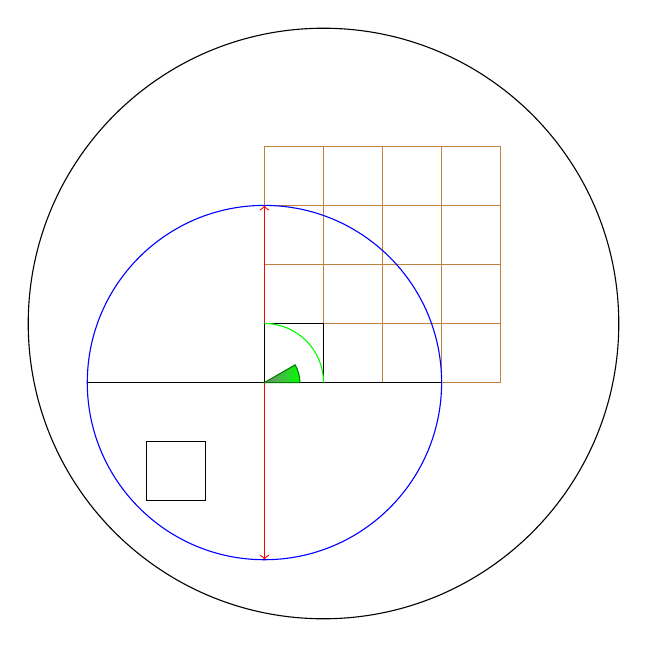
\begin{tikzpicture}[scale=1.5]
\clip[draw] (.5,.5) circle (2.5);
\draw[step=.5cm, gray,color=brown] (0,0) grid (2,2);
\draw (-1.5,0) -- (1.5,0);
\draw [color=red,<->] (0,-1.5) -- (0,1.5);
\draw[color=blue] (0,0) circle (1.5cm);
\draw (0,0) rectangle (0.5,0.5);
\draw (-0.5,-0.5) rectangle (-1,-1);
\draw [color=green] (5mm,0mm) arc (0:90:5mm);
\shadedraw[left color=gray,right color=green, draw=
green!50!black](0,0) -- (3mm,0mm) arc (0:30:3mm) -- cycle;
\end{tikzpicture}
\end{center}
\end{lstlisting}
\end{latin}


\begin{center}
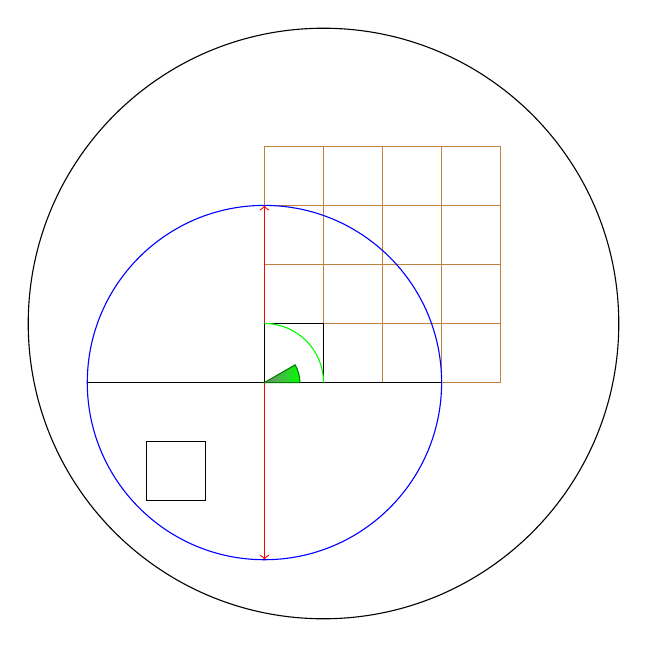
\begin{tikzpicture}[scale=1.5]
\clip[draw] (.5,.5) circle (2.5);
\draw[step=.5cm, gray,color=brown] (0,0) grid (2,2);
\draw (-1.5,0) -- (1.5,0);
\draw [color=red,<->] (0,-1.5) -- (0,1.5);
\draw[color=blue] (0,0) circle (1.5cm);
\draw (0,0) rectangle (0.5,0.5);
\draw (-0.5,-0.5) rectangle (-1,-1);
\draw [color=green] (5mm,0mm) arc (0:90:5mm);
\shadedraw[left color=gray,right color=green, draw=green!50!black](0,0) -- (3mm,0mm) arc (0:30:3mm) -- cycle;
\end{tikzpicture}
\end{center}

اما این همه‌ی هنر این دستور نیست شما تقریبا هر نمودار در فضای ۲بعدی و مختصات دکارتی رامی‌توانید با دستور plot در دستور draw بکشید، برای نمونه می‌توانید دو تا کد زیر و خروجی‌شان را ملاحظه کنید.\footnote{تنها چیزی که لازم است یادآوری کنم این است که دقت کنید هر خط با سمیکولن تمام می‌شود پس اگرانتهای خطی خالی ست بدانید که ادامه دستور در خط بعد آمده، این رااز این بابت گفتم که بتوانید کد رابرای خودتان تشریح کنید}
\begin{center}
\begin{tikzpicture}[scale=.6]
\draw[->] (-7,0) -- (7,0) node[right] {$x$};
\draw[->] (0,-5) -- (0,7) node[above] {$y$};
\draw[color=blue] plot[domain=-6.5:-1.18, samples=70, smooth] (\x, {((\x)^2+1)/((\x)^2-1)}) node[right] {};
\draw[color=blue] plot[domain=1.18:6.5, samples=70, smooth] (\x, {((\x)^2+1)/((\x)^2-1)}) node[right] {};
\draw[color=blue] plot[domain=-.8:.8, samples=70, smooth] (\x, {((\x)^2+1)/((\x)^2-1)}) node[right] {};
\draw[color=blue] plot[domain=-6.5:6.5] (\x, { 1}) node[right] {};
\draw[blue] (1,-4.5) -- (1,6.5) node[above] {};
\draw[blue] (-1,-4.5) -- (-1,6.5) node[above] {};
\fill[blue] (0,-1) circle (.1) (2,1.67) circle (.1) (-2,1.67) circle (.1) (.5,-1.67) circle (.1) (-.5,-1.67) circle (.1) (0,1) circle (.1);
\end{tikzpicture}
\end{center}
\lstset{framexleftmargin=5mm, frame=shadowbox, numbers=left, rulesepcolor=\color{blue}, language=Tex}
\begin{latin}
\begin{lstlisting}[frame=trBL]
\begin{center}
\begin{tikzpicture}[scale=.8]
\draw[->] (-7,0) -- (7,0) node[right] {$x$};
\draw[->] (0,-5) -- (0,7) node[above] {$y$};
\draw[color=blue] plot[domain=-6.5:-1.18, samples=70, smooth] 
(\x, {((\x)^2+1)/((\x)^2-1)}) node[right] {};
\draw[color=blue] plot[domain=1.18:6.5, samples=70, smooth] 
(\x, {((\x)^2+1)/((\x)^2-1)}) node[right] {};
\draw[color=blue] plot[domain=-.8:.8, samples=70, smooth] 
(\x, {((\x)^2+1)/((\x)^2-1)}) node[right] {};
\draw[color=blue] plot[domain=-6.5:6.5] 
(\x,{1}) node[right] {};
\draw[blue] (1,-4.5) -- (1,6.5) node[above] {};
\draw[blue] (-1,-4.5) -- (-1,6.5) node[above] {};
\fill[blue] (0,-1) circle (.1) (2,1.67) circle (.1) 
(-2,1.67) circle (.1) (.5,-1.67) circle (.1) 
(-.5,-1.67) circle (.1) (0,1) circle (.1);
\end{tikzpicture}
\end{center}
\end{lstlisting}
\end{latin}
نمونه‌ی دیگر یک نمودار مثلثاتی ست که تنها یک تفاوت کوچک برای رسمش هست که مختصات رابه رادیان تبدیل می‌کند\footnote{واقعا فکر می‌کنید اگر با گذاشتن کد و خروجی آن را هم می‌گفتم تا زحمت چک کردن هم به خودتان ندهید کار خوبی بود؟!}.
\begin{center}
\begin{tikzpicture}[scale=1, domain=-3.3:3.3]
\draw[->] (-3.5,0) -- (3.5,0) node[right] {$x$};
\draw[->] (0,-5) -- (0,5) node[above] {$y$};
\draw[color=blue] plot[ samples=100, smooth]  (\x, {3*cos(2*\x r)}) node[right] {};
\fill[blue] (-3.14,3) circle (.08) (-1.57,-3) circle (.08) (-.775,0) circle (.08) (0,3) circle (.08) (.775,0) circle (.08) (1.57,-3) circle (.08) (3.14,3) circle (.08);
\draw[blue,dashed] (-1.57,0) -- (-1.57,-3) -- (1.57,-3) -- (1.57,0) (-3.14,0) --(-3.14,3)--(3.14,3)--(3.14,0);
\foreach \x/\xtext in {-3.14/-\pi, -1.57/-\frac{\pi}{2}, -.775/-\frac{\pi}{4}, 0/0, .775/\frac{\pi}{4}, 1.57/\frac{\pi}{2}, 3.14/\pi}
\draw[shift={(\x,0)}] (0pt,0pt) -- (0pt,0pt) node[below] {$\xtext$};
\end{tikzpicture}
\end{center}
\lstset{framexleftmargin=5mm, frame=shadowbox, numbers=left, rulesepcolor=\color{blue}, language=Tex}
\begin{latin}
\begin{lstlisting}[frame=trBL]
\begin{center}
\begin{tikzpicture}[scale=1, domain=-3.3:3.3]
\draw[->] (-3.5,0) -- (3.5,0) node[right] {$x$};
\draw[->] (0,-5) -- (0,5) node[above] {$y$};
\draw[color=blue] plot[ samples=100, smooth] 
(\x, {3*cos(2*\x r)}) node[right] {};
\fill[blue] (-3.14,3) circle (.08) (-1.57,-3) circle (.08)
 (-.775,0) circle (.08) (0,3) circle (.08) 
 (.775,0) circle (.08) (1.57,-3) circle (.08) 
 (3.14,3) circle (.08);
\draw[blue,dashed] (-1.57,0) -- (-1.57,-3) -- (1.57,-3)
 -- (1.57,0) (-3.14,0) --(-3.14,3)--(3.14,3)--(3.14,0);
\foreach \x/\xtext in {-3.14/-\pi, -1.57/-\frac{\pi}{2},
 -.775/-\frac{\pi}{4}, 0/0, .775/\frac{\pi}{4},
  1.57/\frac{\pi}{2}, 3.14/\pi}
\draw[shift={(\x,0)}] (0pt,0pt) -- (0pt,0pt)
 node[below] {$\xtext$};
\end{tikzpicture}
\end{center}
\end{lstlisting}
\end{latin}

\item[fill]
دستور fill هم مشابه دستور draw است، فقط این‌که طبیعتا از آن انتظار داریم همه‌ی اشکال را تو پر بکشد.\footnote{فکر می‌کنم تا همین جا کافی باشد اگر بیشتر از این نمونه خواستید، و از راهنمای tikz نتوانستید استفاده کنید با ما تماس بگیرید، تا در حد توان تجربیات‌مان را تقدیم‌تان کنیم.} البته کاربردش را هم می‌توانید در کدهای بالا ببینید.
\end{description}

\begin{center}
\begin{tikzpicture}[scale=1]
\draw[blue] (.5,0) rectangle (7,4) node[right] {\rl{دانشکده}};
\draw[blue] (2.5,2) circle (1.5) node[] {$A$\ \rl{حسابداری}};
\draw[blue] (5,2) circle (1.5) node[] {$B$\ \rl{مدیریت}};
\end{tikzpicture}

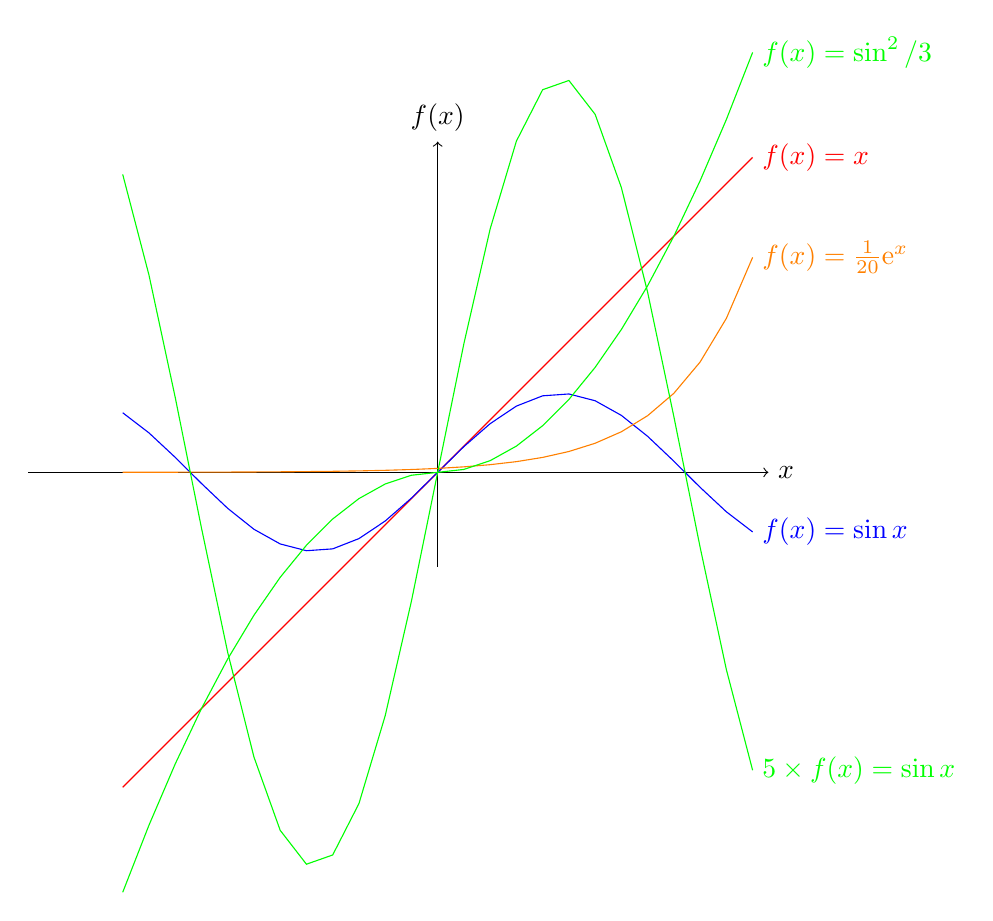
\begin{tikzpicture}[domain=-4:4]
%\draw[very thin,color=gray] (-5,-1.1) grid (9,5);
\draw[->] (-5.2,0) -- (4.2,0) node[right] {$x$};
\draw[->] (0,-1.2) -- (0,4.2) node[above] {$f(x)$};
\draw[color=red] plot (\x,\x) node[right] {$f(x) =x$};
\draw[color=blue] plot (\x,{sin(\x r)}) node[right] {$f(x) = \sin x$};
\draw[color=orange] plot (\x,{0.05*exp(\x)}) node[right] {$f(x) = \frac{1}{20} \mathrm e^x$};
\draw[color=green] plot (\x,{5*sin(\x r)}) node[right] {$5\times f(x) = \sin x$};
\draw[color=green] plot (\x,{(\x^2)/3}) node[right] {$f(x) = \sin^2/ 3$};
\end{tikzpicture}
\end{center}

%\section{بسته tabvar برای رسم جداول تعیین علامت}
%در این قسمت فقط می‌تونید نمونه‌ها رو ببینید، چون واقعا چیز زیادی برا گفتن نداره.
%
%\[\begin{tabvar}{ C|CCCCCCCC} 
%x &-\infty & &1 & &\frac{5}{3}& & +\infty
%\\ \hline
%f'(x)& &+& \barre{0} &- &\barre{0} &+ & &
%\\ \hline
%f(x) &  &\niveau{2}{2}\text{صعودی} &\niveau{0}{ 1}\barre{\text{ماکزیمم}}&\niveau{2}{2}\text{نزولی}&\niveau{0}{1}\barre{\text{مینیمم}}
% &\niveau{2}{2}\text{صعودی}&
%\end{tabvar}\]
%
%\[\begin{tabvar}{C|CCCCCCCCC} 
%x &-\infty & &-1& &0& &+1 & &+\infty 
%\\ \hline
%f'(x) & &+&\barre{0} &-&\dbarre{}&-&\barre{0}&+&
%\\ \hline
%f''(x)& &-&\barre{}&-&\dbarre{}&+&\barre{}&+&
%\\ \hline
%\niveau{2}{2}\TVcenter{f(x)}& &\niveau{2}{2}\TVcenter{\text{صعودی محدب}}&\niveau{0}{1}\barre{\text{ماکزیمم}}&\niveau{2}{2}\TVcenter{\text{نزولی محدب}}&\dbarre{}&\TVcenter{\text{نزولی مقعر}}
%&\niveau{0}{1}\barre{\text{مینیمم}}&\niveau{2}{2}\TVcenter{\text{صعودی مقعر}}&
%\end{tabvar}\]
%
%\[\begin{tabvar}{C|CCCCCCCCC} 
%x &-\infty & &-1& &1& &5& &+\infty \\ \hline
%(1+x)^2& &+&\barre{0}&+&\barre{}&+&\barre{}&+& \\ \hline
%1-x& &+&\barre{}&+&\barre{0}&-&\barre{}&-&\\ \hline
%x-5& & -&\barre{}&-&\barre{}&-&\barre{0}&+&\\ \hline
%f'(x) & &-&\barre{0} &-&\barre{0}&+&\barre{0}&-&\\ \hline
%\niveau{3}{3}\TVcenter{f(x)}& &\decroit &\niveau{0}{2}\barre{}&\niveau{3}{3}\decroit &
%\niveau{0}{2}\barre{\text{مینیمم}}&\niveau{3}{3}\TVcenter{\croit} & \niveau{0}{2}\barre{\text{ماکزیمم}}&\niveau{3}{3}{\decroit} &
%\end{tabvar}\]


\section{رسم گراف}
%\begin{figure}[!ht]
%\centering
%\scalebox{.7}
%{
%\begin{pspicture}(0,0)
%\pscircle[linewidth=.015,dimen=outer](0,0){.4}
%\rput(0,0){$1$}
%\psline[linewidth=.01cm,arrowsize=.1cm,arrowlength=1.5,arrowinset=.2]{-}(-.255,-.255)(-1.15,-1.1)
%\rput(-1.2,-.6){$u_3=0$}
%\psline[linewidth=.01cm,arrowsize=.1cm,arrowlength=1.5,arrowinset=.2]{-}(.26,-.255)(1.2,-1.1)
%\rput(1.6,-.6){$g_3=0$}
%\pscircle[linewidth=.015,dimen=outer](1.4,-1.4){.4}
%\rput(1.4,-1.4){$4$}
%\pscircle[linewidth=.015,dimen=outer](-1.4,-1.4){.4}
%\rput(-1.4,-1.4){$0$}
%\psline[linewidth=.01cm,arrowsize=.1cm,arrowlength=1.5,arrowinset=.2]{-}(-1.65,-1.67)(-2.52,-2.52)
%\pscircle[linewidth=.015,dimen=outer](-2.8,-2.8){.4}
%\rput(-2.8,-2.8){$2$}
%\rput(-2.5,-2){$u_2=0$}
%\psline[linewidth=.01cm,arrowsize=.1cm,arrowlength=1.5,arrowinset=.2]{-}(-2.35,-3.37)(-3.35,-3.37)
%\psline[linewidth=.01cm,arrowsize=.1cm,arrowlength=1.5,arrowinset=.2]{-}(-1.1,-1.65)(-.23,-2.52)
%\rput(0,-2){$g_2=0$}
%\pscircle[linewidth=.015,dimen=outer](0,-2.8){.4}
%\rput(0,-2.8){$3$}
%\end{pspicture} 
%}
%\end{figure}


%\begin{center}
%\begin{tikzpicture}
%\GraphInit[vstyle=Shade]
%\SetVertexNoLabel
%\grTriangularGrid[RA=1,form=2]{6}%
%\end{tikzpicture}
%\end{center}


%\begin{center}
%\begin{tikzpicture}
%\GraphInit[vstyle=Shade]
%\SetVertexLabel
%\grTriangularGrid[prefix=G,Math,RA=1.2]{8}%
%\end{tikzpicture}
%\end{center}
%
%\begin{center}
%\begin{tikzpicture}%
%\GraphInit[vstyle=Art]
%\SetGraphArtColor{black!50}{darkgray}
%\tikzset{VertexStyle/.append style = {
%minimum size = 2pt}}
%\grLCF[RA=3]{1,-3}{4}%
%\end{tikzpicture}
%\end{center}

%\begin{tikzpicture}[scale=1.75]
%\GraphInit[vstyle=Art]
%\Vertex{A}
%\Vertex[x=4,y=0]{B}
%\Vertex[x=1,y=2]{C}
%\Edge[style={bend left}](B)(A)
%\Edges(A,B,C,A)
%\end{tikzpicture}

%\begin{center}
%\begin{tikzpicture}
%\useasboundingbox (-1,-1) rectangle (11,11);
%\tikzset{VertexStyle/.style = {shape = circle,
%ball color = orange,
%text = black,
%inner sep = 2pt,
%outer sep = 0pt,
%minimum size = 24 pt}}
%\tikzset{EdgeStyle/.style = {thick,
%double = orange,
%double distance = 1pt}}
%\tikzset{LabelStyle/.style = {draw,
%fill = yellow,
%text = red}}
%\node[VertexStyle](A){A};
%\node[VertexStyle,right= of A](B){B};
%\node[VertexStyle,right= of B](C){C};
%\node[VertexStyle,above= 7 cm of B](D){D};
%\draw[EdgeStyle](B) to node[LabelStyle]{1} (D) ;
%\tikzset{EdgeStyle/.append style = {bend left}}
%\draw[EdgeStyle](A) to node[LabelStyle]{2} (B);
%\draw[EdgeStyle](B) to node[LabelStyle]{3} (A);
%\draw[EdgeStyle](B) to node[LabelStyle]{4} (C);
%\draw[EdgeStyle](C) to node[LabelStyle]{5} (B);
%\draw[EdgeStyle](A) to node[LabelStyle]{6} (D);
%\draw[EdgeStyle](D) to node[LabelStyle]{7} (C);
%\end{tikzpicture}
%\end{center}

%\begin{tikzpicture}
%\SetGraphUnit{4}
%\Vertex{a}
%\EA(a){b}
%\SO[unit=2](a){c}
%\EA(c){d}
%{\SetGraphUnit{2}
%\SO(c){e}}
%\EA(e){f}
%\Edge(a)(b)
%\tikzset{EdgeStyle/.style = {-,bend left}}
%\Edge(c)(d)
%\tikzset{EdgeStyle/.style = {<->,bend right=90}}
%\Edge(e)(f)
%\end{tikzpicture}

%\begin{tikzpicture}
%\SetVertexNormal[Shape = circle,
%FillColor = orange,
%LineWidth = 2pt]
%\SetUpEdge[lw = 1.5pt,
%color = black,
%labelcolor = white,
%labeltext = red,
%labelstyle = {sloped,draw,text=blue}]
%\Vertex[x=0 ,y=0]{K}
%\Vertex[x=0 ,y=2]{F}
%\Vertex[x=-1,y=4]{D}
%\Vertex[x=3 ,y=7]{H}
%\Vertex[x=8 ,y=5]{B}
%\Vertex[x=9 ,y=2]{N}
%\Vertex[x=5 ,y=0]{M}
%\Vertex[x=3 ,y=1]{S}
%\tikzset{EdgeStyle/.append style = {bend left}}
%\Edge[label = $120$](K)(F)
%\Edge[label = $650$](H)(S)
%\Edge[label = $780$](H)(M)
%\Edge[label = $490$](D)(B)
%\Edge[label = $600$](D)(M)
%\Edge[label = $580$](B)(M)
%\Edge[label = $600$](H)(N)
%\Edge[label = $490$](F)(H)
%\tikzset{EdgeStyle/.append style = {bend right}}
%\Edge[label = $630$](S)(B)
%\Edge[label = $210$](S)(N)
%\Edge[label = $230$](S)(M)
%\end{tikzpicture}

%\begin{tikzpicture}
%\GraphInit[vstyle=Shade]
%\SetGraphUnit{3}
%\Vertex{e}
%\NOEA(e){f}\SOEA(e){d}
%\SOEA(f){h}\NOWE(f){g}
%\WE(g){c} \SOWE(e){a} \SOWE(c){b}
%\tikzstyle{LabelStyle}=[fill=white]
%\tikzstyle{EdgeStyle}=[color=red]
%\Edge[label=$3$](a)(b)
%\Edge[label=$11$](a)(c)
%\Edge[label=$6$](a)(e)
%\Edge[label=$17$](a)(d)
%\Edge[style={pos=.25},label=$20$](a)(g)
%\Edge[label=$5$](c)(b)
%\Edge[label=$6$](c)(e)
%\Edge[label=$7$](c)(g)
%\Edge[label=$7$](f)(e)
%\Edge[label=$3$](d)(e)
%\Edge[label=$9$](d)(h)
%\Edge[label=$6$](g)(e)
%\Edge[style={bend left,out=45,in=135},label=$11$](g)(h)
%\Edge[label=$4$](f)(h)
%\end{tikzpicture}


%\begin{tikzpicture}
%\SetUpEdge[lw = 1.5pt,
%color = orange,
%labelcolor = gray!30,
%labelstyle = {draw}]
%\SetGraphUnit{3}
%\GraphInit[vstyle=Normal]
%\Vertex{P}
%\NOEA(P){B}
%\SOEA(P){M}
%\NOEA(B){D}
%\SOEA(B){C}
%\SOEA(C){L}
%\tikzset{EdgeStyle/.style={->}}
%\Edge[label=$3$](C)(B)
%\Edge[label=$10$](D)(B)
%\Edge[label=$10$](L)(M)
%\Edge[label=$10$](B)(P)
%\tikzset{EdgeStyle/.style={<->}}
%\Edge[label=$4$](P)(M)
%\Edge[label=$9$](C)(M)
%\Edge[label=$4$](C)(L)
%\Edge[label=$5$](C)(D)
%\Edge[label=$10$](B)(M)
%\tikzset{EdgeStyle/.style={<->,relative=false,in=0,out=60}}
%\Edge[label=$11$](L)(D)
%\end{tikzpicture}


\section{الگوریتم}
%\begin{algorithm}[!ht]
% \SetAlgoLined
%\caption{الگوریتم افزایش دوگان.} \label{alg:dualascent}
%برای هر $j$ اندیس $k(j)$ را به صورت زیر تعریف کنید 
%\[
%k(j) = \min\{k\;:\; v_j\leq c_j^k \}.
%\]
%اگر $v_j = c_j^{k(j)}$ آنگاه قرار دهید $k(j) = k(j)+1$. 
%\\
%
%قرار دهید $\text{improvement=true}$.
%\\
%\While{($\text{improvement=true}$)}{
%	قرار دهید 	$\text{improvement=false}$ . 
%	\\
%	\ForEach{$j\in J^+$}{
%قرار دهید $\Delta_j = \min_{i\in I} \{ \rho_i(v) \;:\; v_j-c_{ij}\geq 0 \}$.
%\\
%		\If{$\Delta_j> c_j^{k(j)} -v_j$}{
% قرار دهید $\Delta_j = c_j^{k(j)} -v_j$  .
%\\
%	 					$\text{improvement=true}$.
%	\\
%متغیر $k(j)$ را یک واحد افزایش دهید.
%\\
%            }
%					$v_j$
% را به اندازه‌ی $\Delta_j$ افزایش دهید. (این کار موجب می‌شود که برای هر $i$،  $\rho_i(v)$ به اندازه‌ی $\Delta_j$ کم شود.)
% \\
% }
%} %ENDWHILE
%\end{algorithm}

\renewcommand{\algorithmicif}{\textbf{اگر}}
\renewcommand{\algorithmicthen}{\textbf{آنگاه}}
\renewcommand{\algorithmicelse}{\textbf{وگرنه}}
\renewcommand{\algorithmicprint}{\textbf{چاپ کن}}
\begin{algorithm}[!ht]
\caption{الگوریتم هم‌رنگ‌سازی چندبانده.} \label{alg:multibandblending}
\begin{algorithmic}[1]
\REQUIRE تصاویر $A$ و $B$.\\
\ENSURE تصویر $S$ حاصل از  نیمه‌ی سمت چپ $A$ و نیمه‌ی سمت راست $B$
  \STATE هرمهای لاپلاسین $LA,LB$ از تصاویر $A,B$ ساخته می‌شوند.
  \STATE هرم لاپلاسین سومی به نام $LS$ با کپی کردن نیمه‌های سمت چپ $LA$ و سمت راست $LB$ ساخته می‌شود.
  \STATE تصویر نهایی $S$ با گسترش هر سطح هرم $LS$ و جمع آن با سطح بعدی حاصل خواهد شد.   
  \IF{$mod(a,2)==0$}
  \PRINT $a$ زوج است.
  \ELSE 
  \PRINT $a$ فرد است.  
\ENDIF
\end{algorithmic}
\end{algorithm}


%\renewcommand{\algorithmicif}{\textbf{اگر}}
%\renewcommand{\algorithmicthen}{\textbf{آنگاه}}
%\renewcommand{\algorithmicelse}{\textbf{وگرنه}}
%\renewcommand{\algorithmicprint}{\textbf{چاپ کن}}
\begin{algorithm}[!ht]
\caption{الگوریتم هم‌رنگ‌سازی چندبانده.} \label{alg:multibandblending2}
\begin{algorithmic}[1]
\REQUIRE تصاویر $A$ و $B$.\\
\ENSURE تصویر $S$ حاصل از  نیمه‌ی سمت چپ $A$ و نیمه‌ی سمت راست $B$
  \STATE هرمهای لاپلاسین $LA,LB$ از تصاویر $A,B$ ساخته می‌شوند.
  \STATE هرم لاپلاسین سومی به نام $LS$ با کپی کردن نیمه‌های سمت چپ $LA$ و سمت راست $LB$ ساخته می‌شود.
  \STATE تصویر نهایی $S$ با گسترش هر سطح هرم $LS$ و جمع آن با سطح بعدی حاصل خواهد شد.   
  \IF{$mod(a,2)==0$}
  \PRINT $a$ زوج است.
  \ELSE 
  \PRINT $a$ فرد است.  
\ENDIF
\end{algorithmic}
\end{algorithm}

\begin{algorithm}[!ht]
\caption{الگوریتم برنامه شرالی-آدامز برای دستگاه‌های تساوی}\label{sh-ad}
\begin{algorithmic}[1]
\item[(*)]
ورودی: $ P=\lbrace x \in [0,1]^{n} : Ax=b \rbrace $ و $ k \in [n] $  
\item[(*)]
خروجی: بس‌وجهی  $ A S^{[k]}(p) \subseteq [0,1]^{n} $
  \item[گام 1:]
  هر معادله $ a_{i}x=b_{i} $ را از بس‌وجهی $ P $، در رابطه $ \prod_{i \in I}x_{i} \prod_{j \in J}(1-x_{j}) $، که $ I $ و $ J $ زیرمجموعه‌هایی از $ [n]=\lbrace 1,...,n \rbrace $ هستند، به طوری ‌که $ \vert I \cap J \vert \leq k-1 $ و $  I \cap J = \varnothing $ ضرب کن. یک دستگاه با معادلات چندجمله‌ای به دست می‌آید.  
   \item[گام 2:]
برای همه $ c \in [n] $، هر $ x_{c}^{2}$ را با $ x_{c} $ جایگزین کن. 
    \item[گام 3:]
 همه نامساوی‌های چندجمله‌ای حاصل را اضافه کن.
     \item[گام 4:]
 دستگاه چندجمله‌ای را توسط متغیر $ y_{K} $ برای همه تک جمله‌ای‌های $ \prod_{j \in J}x_{j} $ با $ \vert J \vert \geq 2 $ خطی سازی کن. فرض کنید $ M^{k} $ دستگاه خطی حاصل باشد.
    \item[گام 5:]
قرار بده: $ A S^{[k]}(p):=proj _{X} M^{k} $ که $ X:= \lbrace x_{1},...,x_{n} \rbrace $ 
\end{algorithmic}
\end{algorithm}




%\sout{نمونه}
%
%\xout{نمونه}
%
%\uwave{نمونه}
%
%\uline{نمونه}

\section{جدول}
\[
\rotatebox{50}{
\begin{tabular}{|c|c|c|c|c|}
\hline
ردیف &\multicolumn{4}{|c|}{عنوان}\\
\hline & & & & \\
\hline \multirow{3}{*}{\rotatebox{90}{\mbox{نمونه}}} 
& 1 & نمونه & $\sum$ & $\int$ \\ 
 & 1 & 2 & 3 & 4 \\ 
 & 5 & 6 & 7 & 8 \\ 
\cline{2-5} \multirow{2}{*}{\rotatebox{45}{\mbox{نمونه}}} &  &  &  &  \\ 
  &  &  &  &  \\ 
\hline 
\end{tabular}
}
\]

\begin{table}[!ht]
\centering 
\begin{tabular}{|>{\centering}p{2cm}|>{\centering}p{2cm}|cc} 
 \multicolumn{2}{c}{ \text{شرکت} $I $ } && \\  
\multicolumn{1}{c}{$W$ }  & \multicolumn{1}{c}{$N$  } & &   \\ \cline{1-2}
$16$  \text{و} $-1$ & $14$   
\text{و}
  $14$ & $N$ & \multirow{2}{*}{\text{شرکت}   $J$}\\ \cline{1-2}
$1$  \text{و}
 $-1$  & $ 1$  \text{و}
$ 16$ &$W$ \\ \cline{1-2}
\end{tabular}
\caption{رقابت دو شرکت نفتی}\label{ta1.1}
\end{table}


\begin{tabular}{|p{1.5cm}|>{\raggedright}p{2.5cm}|>{\centering}p{3.5cm}|>{\raggedleft}p{3cm}|}
\hline
پیش‌فرض & چپ-چین & وسط-چین & راست-چین  \tabularnewline
\hline
$1.5$ سانت & $2.5$ سانت & $3.5$ سانت & $3$ سانت \tabularnewline
\hline
\end{tabular}


\begin{longtable}{lll}
\caption{جدول‌های بزرگ با استفاده از بسته \lr{long table}}\\
%\begin{LTR}
   \bfseries Entity&\bfseries  Unicode Name&\bfseries  Unicode\\ \hline
\endfirsthead
%\LTcontcaption{}\\
%   \bfseries Entity&\bfseries  Unicode Name&\bfseries  Unicode\\ \hline
%\endhead
%\LTfincaption{}\\
%   %\bfseries Entity&\bfseries  Unicode Name&\bfseries  Unicode\\ \hline
%\endlasthead
%   %\hline \multicolumn{3}{@{}r@{}}{\emph{Continued on next page}}
%\endfoot
%   %\hline \multicolumn{3}{@{}r@{}}{\emph{Finished on next page}}
%\endprelastfoot
%\noalign{\gdef\Continued{}\gdef\ContTable{}}
%   \hline
\endlastfoot
%\begin{LTR}
alpha              & GREEK SMALL LETTER ALPHA            & 03B1\\
beta               & GREEK SMALL LETTER BETA             & 03B2\\
chi                & GREEK SMALL LETTER CHI              & 03C7\\
\pagebreak
Delta              & GREEK CAPITAL LETTER DELTA          & 0394\\
delta              & GREEK SMALL LETTER DELTA            & 03B4\\
epsi               & GREEK SMALL LETTER EPSILON          & 03B5\\
epsis              & GREEK LUNATE EPSILON SYMBOL         & 03F5\\
epsiv              & GREEK SMALL LETTER EPSILON          & 03B5\\
eta                & GREEK SMALL LETTER ETA              & 03B7\\
Gamma              & GREEK CAPITAL LETTER GAMMA          & 0393\\
gamma              & GREEK SMALL LETTER GAMMA            & 03B3\\
gammad             & GREEK SMALL LETTER DIGAMMA          & 03DD\\
iota               & GREEK SMALL LETTER IOTA             & 03B9\\
kappa              & GREEK SMALL LETTER KAPPA            & 03BA\\
kappav             & GREEK KAPPA SYMBOL                  & 03F0\\
Lambda             & GREEK CAPITAL LETTER LAMDA          & 039B\\
lambda             & GREEK SMALL LETTER LAMDA            & 03BB\\
mu                 & GREEK SMALL LETTER MU               & 03BC\\
nu                 & GREEK SMALL LETTER NU               & 03BD\\
Omega              & GREEK CAPITAL LETTER OMEGA          & 03A9\\
omega              & GREEK SMALL LETTER OMEGA            & 03C9\\
Phi                & GREEK CAPITAL LETTER PHI            & 03A6\\
phis               & GREEK PHI SYMBOL                    & 03D5\\
phiv               & GREEK SMALL LETTER PHI              & 03C6\\
Pi                 & GREEK CAPITAL LETTER PI             & 03A0\\
pi                 & GREEK SMALL LETTER PI               & 03C0\\
piv                & GREEK PI SYMBOL                     & 03D6\\
Psi                & GREEK CAPITAL LETTER PSI            & 03A8\\
psi                & GREEK SMALL LETTER PSI              & 03C8\\
rho                & GREEK SMALL LETTER RHO              & 03C1\\
rhov               & GREEK RHO SYMBOL                    & 03F1\\
Sigma              & GREEK CAPITAL LETTER SIGMA          & 03A3\\
sigma              & GREEK SMALL LETTER SIGMA            & 03C3\\
sigmav             & GREEK SMALL LETTER FINAL SIGMA      & 03C2\\
tau                & GREEK SMALL LETTER TAU              & 03C4\\
Theta              & GREEK CAPITAL LETTER THETA          & 0398\\
thetas             & GREEK SMALL LETTER THETA            & 03B8\\
thetav             & GREEK THETA SYMBOL                  & 03D1\\
Upsi               & GREEK UPSILON WITH HOOK SYMBOL      & 03D2\\
upsi               & GREEK SMALL LETTER UPSILON          & 03C5\\
Xi                 & GREEK CAPITAL LETTER XI             & 039E\\
xi                 & GREEK SMALL LETTER XI               & 03BE\\
zeta               & GREEK SMALL LETTER ZETA             & 03B6\\
%
%
%
alpha              &  SMALL LETTER ALPHA            & 03B1\\
beta               &  SMALL LETTER BETA             & 03B2\\
chi                &  SMALL LETTER CHI              & 03C7\\
Delta              &  CAPITAL LETTER DELTA          & 0394\\
delta              &  SMALL LETTER DELTA            & 03B4\\
epsi               &  SMALL LETTER EPSILON          & 03B5\\
epsis              &  LUNATE EPSILON SYMBOL         & 03F5\\
epsiv              &  SMALL LETTER EPSILON          & 03B5\\
eta                &  SMALL LETTER ETA              & 03B7\\
Gamma              &  CAPITAL LETTER GAMMA          & 0393\\
gamma              &  SMALL LETTER GAMMA            & 03B3\\
gammad             &  SMALL LETTER DIGAMMA          & 03DD\\
iota               &  SMALL LETTER IOTA             & 03B9\\
kappa              &  SMALL LETTER KAPPA            & 03BA\\
kappav             &  KAPPA SYMBOL                  & 03F0\\
Lambda             &  CAPITAL LETTER LAMDA          & 039B\\
lambda             &  SMALL LETTER LAMDA            & 03BB\\
mu                 &  SMALL LETTER MU               & 03BC\\
nu                 &  SMALL LETTER NU               & 03BD\\
Omega              &  CAPITAL LETTER OMEGA          & 03A9\\
omega              &  SMALL LETTER OMEGA            & 03C9\\
Phi                &  CAPITAL LETTER PHI            & 03A6\\
phis               &  PHI SYMBOL                    & 03D5\\
phiv               &  SMALL LETTER PHI              & 03C6\\
Pi                 &  CAPITAL LETTER PI             & 03A0\\
pi                 &  SMALL LETTER PI               & 03C0\\
piv                &  PI SYMBOL                     & 03D6\\
Psi                &  CAPITAL LETTER PSI            & 03A8\\
psi                &  SMALL LETTER PSI              & 03C8\\
rho                &  SMALL LETTER RHO              & 03C1\\
rhov               &  RHO SYMBOL                    & 03F1\\
Sigma              &  CAPITAL LETTER SIGMA          & 03A3\\
sigma              &  SMALL LETTER SIGMA            & 03C3\\
sigmav             &  SMALL LETTER FINAL SIGMA      & 03C2\\
tau                &  SMALL LETTER TAU              & 03C4\\
Theta              &  CAPITAL LETTER THETA          & 0398\\
thetas             &  SMALL LETTER THETA            & 03B8\\
thetav             &  THETA SYMBOL                  & 03D1\\
Upsi               &  UPSILON WITH HOOK SYMBOL      & 03D2\\
upsi               &  SMALL LETTER UPSILON          & 03C5\\
Xi                 &  CAPITAL LETTER XI             & 039E\\
xi                 &  SMALL LETTER XI               & 03BE\\
zeta               &  SMALL LETTER ZETA             & 03B6\\
%
%
%
alpha              &  SMALL LETTER ALPHA            & 03B1\\
beta               &  SMALL LETTER BETA             & 03B2\\
chi                &  SMALL LETTER CHI              & 03C7\\
Delta              &  CAPITAL LETTER DELTA          & 0394\\
delta              &  SMALL LETTER DELTA            & 03B4\\
epsi               &  SMALL LETTER EPSILON          & 03B5\\
epsis              &  LUNATE EPSILON SYMBOL         & 03F5\\
epsiv              &  SMALL LETTER EPSILON          & 03B5\\
eta                &  SMALL LETTER ETA              & 03B7\\
Gamma              &  CAPITAL LETTER GAMMA          & 0393\\
gamma              &  SMALL LETTER GAMMA            & 03B3\\
gammad             &  SMALL LETTER DIGAMMA          & 03DD\\
iota               &  SMALL LETTER IOTA             & 03B9\\
kappa              &  SMALL LETTER KAPPA            & 03BA\\
kappav             &  KAPPA SYMBOL                  & 03F0\\
Lambda             &  CAPITAL LETTER LAMDA          & 039B\\
lambda             &  SMALL LETTER LAMDA            & 03BB\\
mu                 &  SMALL LETTER MU               & 03BC\\
nu                 &  SMALL LETTER NU               & 03BD\\
Omega              &  CAPITAL LETTER OMEGA          & 03A9\\
omega              &  SMALL LETTER OMEGA            & 03C9\\
Phi                &  CAPITAL LETTER PHI            & 03A6\\
phis               &  PHI SYMBOL                    & 03D5\\
phiv               &  SMALL LETTER PHI              & 03C6\\
Pi                 &  CAPITAL LETTER PI             & 03A0\\
pi                 &  SMALL LETTER PI               & 03C0\\
piv                &  PI SYMBOL                     & 03D6\\
Psi                &  CAPITAL LETTER PSI            & 03A8\\
psi                &  SMALL LETTER PSI              & 03C8\\
rho                &  SMALL LETTER RHO              & 03C1\\
rhov               &  RHO SYMBOL                    & 03F1\\
Sigma              &  CAPITAL LETTER SIGMA          & 03A3\\
sigma              &  SMALL LETTER SIGMA            & 03C3\\
sigmav             &  SMALL LETTER FINAL SIGMA      & 03C2\\
tau                &  SMALL LETTER TAU              & 03C4\\
Theta              &  CAPITAL LETTER THETA          & 0398\\
thetas             &  SMALL LETTER THETA            & 03B8\\
thetav             &  THETA SYMBOL                  & 03D1\\
Upsi               &  UPSILON WITH HOOK SYMBOL      & 03D2\\
upsi               &  SMALL LETTER UPSILON          & 03C5\\
Xi                 &  CAPITAL LETTER XI             & 039E\\
xi                 &  SMALL LETTER XI               & 03BE\\
zeta               &  SMALL LETTER ZETA             & 03B6\\
%
%
%
alpha              &  SMALL LETTER ALPHA            & 03B1\\
beta               &  SMALL LETTER BETA             & 03B2\\
chi                &  SMALL LETTER CHI              & 03C7\\
Delta              &  CAPITAL LETTER DELTA          & 0394\\
delta              &  SMALL LETTER DELTA            & 03B4\\
epsi               &  SMALL LETTER EPSILON          & 03B5\\
epsis              &  LUNATE EPSILON SYMBOL         & 03F5\\
epsiv              &  SMALL LETTER EPSILON          & 03B5\\
eta                &  SMALL LETTER ETA              & 03B7\\
Gamma              &  CAPITAL LETTER GAMMA          & 0393\\
gamma              &  SMALL LETTER GAMMA            & 03B3\\
gammad             &  SMALL LETTER DIGAMMA          & 03DD\\
iota               &  SMALL LETTER IOTA             & 03B9\\
kappa              &  SMALL LETTER KAPPA            & 03BA\\
kappav             &  KAPPA SYMBOL                  & 03F0\\
Lambda             &  CAPITAL LETTER LAMDA          & 039B\\
lambda             &  SMALL LETTER LAMDA            & 03BB\\
mu                 &  SMALL LETTER MU               & 03BC\\
nu                 &  SMALL LETTER NU               & 03BD\\
Omega              &  CAPITAL LETTER OMEGA          & 03A9\\
omega              &  SMALL LETTER OMEGA            & 03C9\\
Phi                &  CAPITAL LETTER PHI            & 03A6\\
phis               &  PHI SYMBOL                    & 03D5\\
phiv               &  SMALL LETTER PHI              & 03C6\\
Pi                 &  CAPITAL LETTER PI             & 03A0\\
pi                 &  SMALL LETTER PI               & 03C0\\
piv                &  PI SYMBOL                     & 03D6\\
Psi                &  CAPITAL LETTER PSI            & 03A8\\
psi                &  SMALL LETTER PSI              & 03C8\\
rho                &  SMALL LETTER RHO              & 03C1\\
rhov               &  RHO SYMBOL                    & 03F1\\
Sigma              &  CAPITAL LETTER SIGMA          & 03A3\\
sigma              &  SMALL LETTER SIGMA            & 03C3\\
sigmav             &  SMALL LETTER FINAL SIGMA      & 03C2\\
tau                &  SMALL LETTER TAU              & 03C4\\
Theta              &  CAPITAL LETTER THETA          & 0398\\
thetas             &  SMALL LETTER THETA            & 03B8\\
thetav             &  THETA SYMBOL                  & 03D1\\
Upsi               &  UPSILON WITH HOOK SYMBOL      & 03D2\\
upsi               &  SMALL LETTER UPSILON          & 03C5\\
Xi                 &  CAPITAL LETTER XI             & 039E\\
xi                 &  SMALL LETTER XI               & 03BE\\
zeta               &  SMALL LETTER ZETA             & 03B6\\
%\end{LTR}
\end{longtable}



%\begin{longtable}{|c|c|c|c|c|c|c|c|c|}\hline
%0.1 & 2. & 5. & 0.01 & 0.5 & 0.6814 & 0.2322 & 0.4492 & 0.6592 \\\hline 
%0.1 & 2. & 5. & 0.01 & 1. & 0.6814 & 0.3425 & 0.3389 & 0.4974 \\\hline 
%0.1 & 2. & 5. & 0.01 & 1.5 & 0.6814 & 0.4089 & 0.2725 & 0.3999 \\\hline 
%0.1 & 2. & 5. & 0.01 & 2. & 0.6814 & 0.4536 & 0.2278 & 0.3343 \\\hline 
%0.1 & 2. & 5. & 0.01 & 2.5 & 0.6814 & 0.4857 & 0.1957 & 0.2872 \\\hline 
%0.1 & 2. & 5. & 0.01 & 3. & 0.6814 & 0.51 & 0.1714 & 0.2515 \\\hline 
%0.1 & 2. & 5. & 0.01 & 3.5 & 0.6814 & 0.529 & 0.1524 & 0.2237 \\\hline 
%0.1 & 2. & 5. & 0.01 & 4. & 0.6814 & 0.5442 & 0.1372 & 0.2014 \\\hline 
%0.1 & 2. & 5. & 0.01 & 4.5 & 0.6814 & 0.5567 & 0.1247 & 0.183 \\\hline 
%0.1 & 2. & 5. & 0.01 & 5. & 0.6814 & 0.5671 & 0.1143 & 0.1677 \\\hline 
%0.1 & 2. & 5. & 0.04 & 1. & 0.6758 & 0.3366 & 0.3391 & 0.5019 \\\hline 
%0.1 & 2. & 5. & 0.04 & 1.5 & 0.6758 & 0.4027 & 0.273 & 0.404 \\\hline 
%0.1 & 2. & 5. & 0.04 & 2. & 0.6758 & 0.4473 & 0.2285 & 0.3381 \\\hline 
%0.1 & 2. & 5. & 0.04 & 2.5 & 0.6758 & 0.4794 & 0.1963 & 0.2905 \\\hline 
%0.1 & 2. & 5. & 0.04 & 3. & 0.6758 & 0.5037 & 0.1721 & 0.2546 \\\hline 
%0.1 & 2. & 5. & 0.04 & 3.5 & 0.6758 & 0.5227 & 0.1531 & 0.2265 \\\hline 
%0.1 & 2. & 5. & 0.04 & 4. & 0.6758 & 0.5379 & 0.1378 & 0.204 \\\hline 
%0.1 & 2. & 5. & 0.04 & 4.5 & 0.6758 & 0.5504 & 0.1253 & 0.1855 \\\hline 
%0.1 & 2. & 5. & 0.04 & 5. & 0.6758 & 0.5609 & 0.1149 & 0.17 \\\hline 
%0.1 & 2. & 5. & 0.07 & 0.5 & 0.6701 & 0.2223 & 0.4478 & 0.6683 \\\hline 
%0.1 & 2. & 5. & 0.07 & 1. & 0.6701 & 0.3307 & 0.3394 & 0.5065 \\\hline 
%0.1 & 2. & 5. & 0.07 & 1.5 & 0.6701 & 0.3965 & 0.2736 & 0.4083 \\\hline 
%0.1 & 2. & 5. & 0.07 & 2. & 0.6701 & 0.441 & 0.2291 & 0.3419 \\\hline 
%0.1 & 2. & 5. & 0.07 & 2.5 & 0.6701 & 0.4731 & 0.197 & 0.294 \\\hline 
%0.1 & 2. & 5. & 0.07 & 3. & 0.6701 & 0.4973 & 0.1728 & 0.2578 \\\hline 
%0.1 & 2. & 5. & 0.07 & 3.5 & 0.6701 & 0.5163 & 0.1538 & 0.2295 \\\hline 
%0.1 & 2. & 5. & 0.07 & 4. & 0.6701 & 0.5316 & 0.1385 & 0.2067 \\\hline 
%0.1 & 2. & 5. & 0.07 & 4.5 & 0.6701 & 0.5441 & 0.1259 & 0.188 \\\hline 
%0.1 & 2. & 5. & 0.07 & 5. & 0.6701 & 0.5546 & 0.1155 & 0.1723 \\\hline 
%0.1 & 2. & 5. & 0.1 & 0.5 & 0.6644 & 0.2173 & 0.447 & 0.6729 \\\hline 
%0.1 & 2. & 5. & 0.1 & 1. & 0.6644 & 0.3248 & 0.3396 & 0.5112 \\\hline 
%0.1 & 2. & 5. & 0.1 & 1.5 & 0.6644 & 0.3903 & 0.2741 & 0.4126 \\\hline 
%0.1 & 2. & 5. & 0.1 & 2. & 0.6644 & 0.4346 & 0.2298 & 0.3458 \\\hline 
%0.1 & 2. & 5. & 0.1 & 2.5 & 0.6644 & 0.4666 & 0.1977 & 0.2976 \\\hline 
%0.1 & 2. & 5. & 0.1 & 3. & 0.6644 & 0.4909 & 0.1734 & 0.2611 \\\hline 
%0.1 & 2. & 5. & 0.1 & 3.5 & 0.6644 & 0.5099 & 0.1544 & 0.2324 \\\hline 
%0.1 & 2. & 5. & 0.1 & 4. & 0.6644 & 0.5252 & 0.1391 & 0.2094 \\\hline 
%0.1 & 2. & 5. & 0.1 & 4.5 & 0.6644 & 0.5378 & 0.1266 & 0.1905 \\\hline 
%0.1 & 2. & 5. & 0.1 & 5. & 0.6644 & 0.5483 & 0.1161 & 0.1747 \\\hline 
%0.1 & 2. & 5. & 0.13 & 1. & 0.6586 & 0.3188 & 0.3398 & 0.5159 \\\hline 
%0.1 & 2. & 5. & 0.13 & 1.5 & 0.6586 & 0.3839 & 0.2746 & 0.417 \\\hline 
%0.1 & 2. & 5. & 0.13 & 2. & 0.6586 & 0.4282 & 0.2304 & 0.3499 \\\hline 
%0.1 & 2. & 5. & 0.13 & 2.5 & 0.6586 & 0.4602 & 0.1984 & 0.3012 \\\hline 
%0.1 & 2. & 5. & 0.13 & 3. & 0.6586 & 0.4844 & 0.1741 & 0.2644 \\\hline 
%0.1 & 2. & 5. & 0.13 & 3.5 & 0.6586 & 0.5035 & 0.1551 & 0.2355 \\\hline 
%0.1 & 2. & 5. & 0.13 & 4. & 0.6586 & 0.5188 & 0.1398 & 0.2122 \\\hline 
%0.1 & 2. & 5. & 0.13 & 4.5 & 0.6586 & 0.5314 & 0.1272 & 0.1931 \\\hline 
%0.1 & 2. & 5. & 0.13 & 5. & 0.6586 & 0.5419 & 0.1167 & 0.1771 \\\hline 
%0.1 & 2. & 5. & 0.16 & 0.5 & 0.6527 & 0.2073 & 0.4454 & 0.6823 \\\hline 
%0.1 & 2. & 5. & 0.16 & 1. & 0.6527 & 0.3128 & 0.3399 & 0.5208 \\\hline 
%0.1 & 2. & 5. & 0.16 & 1.5 & 0.6527 & 0.3776 & 0.2751 & 0.4215 \\\hline 
%0.1 & 2. & 5. & 0.16 & 2. & 0.6527 & 0.4217 & 0.231 & 0.354 \\\hline 
%0.1 & 2. & 5. & 0.16 & 2.5 & 0.6527 & 0.4536 & 0.1991 & 0.305 \\\hline 
%0.1 & 2. & 5. & 0.16 & 3. & 0.6527 & 0.4779 & 0.1748 & 0.2678 \\\hline 
%0.1 & 2. & 5. & 0.16 & 3.5 & 0.6527 & 0.4969 & 0.1558 & 0.2386 \\\hline 
%0.1 & 2. & 5. & 0.16 & 4. & 0.6527 & 0.5123 & 0.1404 & 0.2151 \\\hline 
%0.1 & 2. & 5. & 0.16 & 4.5 & 0.6527 & 0.5249 & 0.1278 & 0.1958 \\\hline 
%0.1 & 2. & 5. & 0.16 & 5. & 0.6527 & 0.5354 & 0.1173 & 0.1796 \\\hline 
%0.1 & 2. & 5. & 0.19 & 0.5 & 0.6468 & 0.2023 & 0.4445 & 0.6872 \\\hline 
%0.1 & 2. & 5. & 0.19 & 1. & 0.6468 & 0.3067 & 0.3401 & 0.5258 \\\hline 
%0.1 & 2. & 5. & 0.19 & 1.5 & 0.6468 & 0.3712 & 0.2756 & 0.4261 \\\hline 
%0.1 & 2. & 5. & 0.19 & 2. & 0.6468 & 0.4151 & 0.2317 & 0.3582 \\\hline 
%0.1 & 2. & 5. & 0.19 & 2.5 & 0.6468 & 0.447 & 0.1997 & 0.3088 \\\hline 
%0.1 & 2. & 5. & 0.19 & 3. & 0.6468 & 0.4713 & 0.1755 & 0.2713 \\\hline 
%0.1 & 2. & 5. & 0.19 & 3.5 & 0.6468 & 0.4903 & 0.1564 & 0.2419 \\\hline 
%0.1 & 2. & 5. & 0.19 & 4. & 0.6468 & 0.5057 & 0.1411 & 0.2181 \\\hline 
%0.1 & 2. & 5. & 0.19 & 4.5 & 0.6468 & 0.5183 & 0.1284 & 0.1986 \\\hline 
%0.1 & 2. & 5. & 0.19 & 5. & 0.6468 & 0.5289 & 0.1179 & 0.1822 \\\hline 
%0.1 & 2. & 5. & 0.19 & 5. & 0.6468 & 0.5289 & 0.1179 & 0.1822 \\\hline 
%2.3 & 2. & 5. & 0.01 & 1.5 & 0.7664 & 0.4294 & 0.337 & 0.4397 \\\hline 
%2.3 & 2. & 5. & 0.01 & 2. & 0.7664 & 0.4833 & 0.2831 & 0.3694 \\\hline 
%2.3 & 2. & 5. & 0.01 & 2.5 & 0.7664 & 0.528 & 0.2384 & 0.3111 \\\hline 
%2.3 & 2. & 5. & 0.01 & 3. & 0.7664 & 0.5521 & 0.2142 & 0.2795 \\\hline 
%2.3 & 2. & 5. & 0.01 & 3.5 & 0.7664 & 0.5755 & 0.1909 & 0.2491 \\\hline 
%2.3 & 2. & 5. & 0.01 & 4. & 0.7664 & 0.5943 & 0.1721 & 0.2246 \\\hline 
%2.3 & 2. & 5. & 0.01 & 4.5 & 0.7664 & 0.6097 & 0.1566 & 0.2044 \\\hline 
%2.3 & 2. & 5. & 0.01 & 5. & 0.7664 & 0.6227 & 0.1437 & 0.1875 \\\hline 
%2.3 & 2. & 5. & 0.04 & 0.5 & 0.5747 & 0.0881 & 0.4866 & 0.8466 \\\hline 
%2.3 & 2. & 5. & 0.04 & 1. & 0.5747 & 0.1764 & 0.3984 & 0.6931 \\\hline 
%2.3 & 2. & 5. & 0.04 & 1.5 & 0.5747 & 0.2361 & 0.3386 & 0.5892 \\\hline 
%3. & 2. & 2. & 0.01 & 0.5 & 1.4156 & 0.5655 & 0.8501 & 0.6005 \\\hline 
%3. & 2. & 2. & 0.01 & 1. & 1.4156 & 0.7939 & 0.6217 & 0.4392 \\\hline 
%3. & 2. & 2. & 0.01 & 1.5 & 1.4156 & 0.9248 & 0.4907 & 0.3467 \\\hline 
%3. & 2. & 2. & 0.01 & 2. & 1.4156 & 1.0101 & 0.4055 & 0.2864 \\\hline 
%3. & 2. & 2. & 0.01 & 2.5 & 1.4156 & 1.0701 & 0.3455 & 0.2441 \\\hline 
%3. & 2. & 2. & 0.01 & 3. & 1.4156 & 1.1146 & 0.301 & 0.2126 \\\hline 
%3. & 2. & 2. & 0.01 & 3.5 & 1.4156 & 1.149 & 0.2666 & 0.1883 \\\hline 
%3. & 2. & 2. & 0.01 & 4. & 1.4156 & 1.1763 & 0.2393 & 0.169 \\\hline 
%3. & 2. & 2. & 0.01 & 4.5 & 1.4156 & 1.1985 & 0.217 & 0.1533 \\\hline 
%3. & 2. & 2. & 0.01 & 5. & 1.4156 & 1.217 & 0.1986 & 0.1403 \\\hline 
%3. & 2. & 2. & 0.04 & 0.5 & 1.2221 & 0.4173 & 0.8049 & 0.6586 \\\hline 
%3. & 2. & 2. & 0.04 & 1. & 1.2221 & 0.616 & 0.6061 & 0.496 \\\hline 
%3. & 2. & 2. & 0.04 & 1.5 & 1.2221 & 0.7353 & 0.4868 & 0.3983 \\\hline 
%3. & 2. & 2. & 0.04 & 2. & 1.2221 & 0.8152 & 0.4069 & 0.333 \\\hline 
%3. & 2. & 2. & 0.04 & 2.5 & 1.2221 & 0.8724 & 0.3497 & 0.2861 \\\hline 
%3. & 2. & 2. & 0.04 & 3. & 1.2221 & 0.9155 & 0.3066 & 0.2509 \\\hline 
%3. & 2. & 2. & 0.04 & 3.5 & 1.2221 & 0.9491 & 0.273 & 0.2234 \\\hline 
%3. & 2. & 2. & 0.04 & 4. & 1.2221 & 0.976 & 0.2461 & 0.2014 \\\hline 
%3. & 2. & 2. & 0.04 & 4.5 & 1.2221 & 0.9981 & 0.224 & 0.1833 \\\hline 
%3. & 2. & 2. & 0.04 & 5. & 1.2221 & 1.0166 & 0.2055 & 0.1682 \\\hline 
%3. & 2. & 2. & 0.07 & 0.5 & 1.0032 & 0.2681 & 0.7351 & 0.7328 \\\hline 
%3. & 2. & 2. & 0.07 & 1. & 1.0032 & 0.4276 & 0.5756 & 0.5737 \\\hline 
%3. & 2. & 2. & 0.07 & 1.5 & 1.0032 & 0.53 & 0.4732 & 0.4717 \\\hline 
%3. & 2. & 2. & 0.07 & 2. & 1.0032 & 0.6012 & 0.402 & 0.4008 \\\hline 
%3. & 2. & 2. & 0.07 & 2.5 & 1.0032 & 0.6535 & 0.3497 & 0.3485 \\\hline 
%3. & 2. & 2. & 0.07 & 3. & 1.0032 & 0.6937 & 0.3095 & 0.3085 \\\hline 
%3. & 2. & 2. & 0.07 & 3.5 & 1.0032 & 0.7256 & 0.2776 & 0.2767 \\\hline 
%3. & 2. & 2. & 0.07 & 4. & 1.0032 & 0.7515 & 0.2517 & 0.2509 \\\hline 
%3. & 2. & 2. & 0.07 & 4.5 & 1.0032 & 0.7729 & 0.2303 & 0.2296 \\\hline 
%3. & 2. & 2. & 0.07 & 5. & 1.0032 & 0.791 & 0.2122 & 0.2116 \\\hline 
%3. & 2. & 2. & 0.1 & 0.5 & 0.7525 & 0.1283 & 0.6241 & 0.8294 \\\hline 
%3. & 2. & 2. & 0.1 & 1. & 0.7525 & 0.2361 & 0.5164 & 0.6863 \\\hline 
%3. & 2. & 2. & 0.1 & 1.5 & 0.7525 & 0.313 & 0.4394 & 0.584 \\\hline 
%3. & 2. & 2. & 0.1 & 2. & 0.7525 & 0.37 & 0.3825 & 0.5083 \\\hline 
%3. & 2. & 2. & 0.1 & 2.5 & 0.7525 & 0.4137 & 0.3387 & 0.4502 \\\hline 
%3. & 2. & 2. & 0.1 & 3. & 0.7525 & 0.4484 & 0.3041 & 0.4041 \\\hline 
%3. & 2. & 2. & 0.1 & 3.5 & 0.7525 & 0.4765 & 0.2759 & 0.3667 \\\hline 
%3. & 2. & 2. & 0.1 & 4. & 0.7525 & 0.4999 & 0.2526 & 0.3357 \\\hline 
%3. & 2. & 2. & 0.1 & 4.5 & 0.7525 & 0.5195 & 0.233 & 0.3096\\\hline
%\end{longtable}

\clearpage
\subsection{بسته array}
تنظیمات جالبی برای مدیریت جدول هاوجود دارد که با استفاده از بسته ی array‌ می‌توان به آن‌ها دست پیدا کرد. این بسته امکان اعمال تغییرات ستونی را برای ما فراهم می‌کند.

\begin{table}[h!]
\centering
\begin{tabular}{|>{\tiny} p{1cm}|>{\large\it\bf} b{2cm}|>\Large m{3cm}|}
\hline
1 1 1 1 1 1  1 1 1 1 1 1  1 1 1 1 1 1  1 1 1 1 1 1  &
2 2 2 2 2 2 2 2 2 2 2 2 2 2 2 2 2 2 2 2 2 2 2 2  2 &
3 3 3 3 3 3 3 3 3 3 3 3 3 3 3 3 3 3 3 3 3 3 3 3 3 \\
\hline
1 1 1 1 1 1  1 1 1 1 1 1  1 1 1 1 1 1  1 1 1 1 1 1  &
2 2 2 2 2 2 2 2 2 2 2 2 2 2 2 2 2 2 2 2 2 2 2 2  2 &
3 3 3 3 3 3 3 3 3 3 3 3 3 3 3 3 3 3 3 3 3 3 3 3 3 \\
\hline
\end{tabular}
\end{table}
